% =====================================================================
% ICAST-ES (ISAS) 2026 submission — DOUBLE-BLIND (anonim).
% Template: IEEE conference (IEEEtran). Untuk IEIT Polinema: lepas anonim
% (isi \author{} dgn nama+afiliasi) — sisanya sama.
% Build: pdflatex main && bibtex main && pdflatex main && pdflatex main
% TODO sebelum submit: angka [CONFIRM], detail dataset, sitasi [CEK] di refs.bib.
% =====================================================================
\documentclass[conference]{IEEEtran}
\IEEEoverridecommandlockouts
\usepackage{cite}
\usepackage{amsmath,amssymb,amsfonts}
\usepackage{graphicx}
\usepackage{booktabs}
\usepackage{xcolor}
\usepackage{url}
\usepackage[hidelinks]{hyperref}

\begin{document}

\title{Canonical Alignment and Angular-Margin Learning for\\
Robust 3D Palm Recognition with PointNet++}

% --- DOUBLE-BLIND: jangan cantumkan identitas. Untuk IEIT, ganti blok ini. ---
\author{\IEEEauthorblockN{Anonymous Author(s)}
\IEEEauthorblockA{\textit{Affiliation withheld for double-blind review}}}

\maketitle

\begin{abstract}
Contactless 3D palm recognition is attractive for hygienic, hard-to-spoof
biometrics, yet point-cloud backbones such as PointNet++ have been reported to
perform weakly on hand modalities. We revisit this setting with two coupled
factors and isolate their effects through a full factorial study:
\emph{point-cloud canonicalization} and \emph{angular-margin learning}. Using a
single shared PointNet++ encoder, we evaluate six representations
(raw, centering, center+scale, PCA-canonical, deterministic PCA-robust, and an
anatomical landmark frame) crossed with two loss configurations (cosine softmax
and ArcFace), across five seeds under a closed-set protocol with a held-out probe
set and multi-frame fusion. We show that (i) canonicalization is decisive for
rotation robustness, but \emph{not all} normalizations help: plain PCA exhibits a
sharp axis-assignment singularity at $90^{\circ}$, which our deterministic
PCA-robust variant removes, yielding a flat error profile across rotations; and
(ii) angular margin substantially improves class separability on every
normalized representation---roughly doubling the discriminability index
$d'$ (all $p<0.05$, paired test over seeds)---while the equal-error rate (EER)
saturates near zero at the operating point and therefore understates the effect.
The full pipeline reaches an EER of $0.0$--$0.5\%$ under canonicalization,
contradicting the view that PointNet++ is weak for hand biometrics.
\end{abstract}

\begin{IEEEkeywords}
3D palm recognition, point cloud, PointNet++, ArcFace, angular margin, metric
learning, canonicalization, rotation robustness, biometrics.
\end{IEEEkeywords}

% =====================================================================
\section{Introduction}
% =====================================================================
Hand-based biometrics are convenient and socially accepted, and contactless 3D
acquisition (e.g., structured-light/time-of-flight depth on consumer devices)
avoids the hygiene and latent-print concerns of contact sensors. A depth scan of
the palm can be back-projected into a 3D point cloud, which preserves the
surface geometry of the palm and fingers. However, prior studies that applied
point-cloud networks such as PointNet/PointNet++ to hand or palm modalities
reported only moderate accuracy, suggesting that such backbones are not
competitive for this task~\cite{svoboda2020palm,zhang2023palm3d}.

We argue that this conclusion conflates the \emph{backbone} with two design
choices that are usually left implicit: how the point cloud is
\emph{canonicalized} before it enters the network, and which \emph{loss} shapes
the embedding space. To disentangle them we adopt a factorial design and measure
all combinations of six alignment variants and two loss configurations, with the
\emph{same} PointNet++ encoder, so that each conclusion holds \emph{across} the
other factor rather than at a single hand-picked setting.

\noindent\textbf{Contributions.}
\begin{itemize}
\item A \emph{deterministic PCA-robust canonicalization} that removes the
$90^{\circ}$ axis-assignment singularity of plain PCA alignment, giving a flat
error profile under in-plane rotation (our primary methodological contribution).
\item A controlled, anti-circular \emph{factorial} evaluation
(alignment\,$\times$\,loss, five seeds) showing that angular margin improves
embedding separability on \emph{every} normalized representation, evidenced
through $d'$ rather than a floored EER.
\item Evidence that a pure PointNet++ pipeline reaches near-zero EER for 3D palm
recognition, contradicting prior ``PointNet++ is weak'' findings.
\end{itemize}

% =====================================================================
\section{Related Work}
% =====================================================================
\textbf{Point-cloud deep learning.} PointNet~\cite{qi2017pointnet} processes
unordered point sets with shared MLPs and a symmetric pooling function;
PointNet++~\cite{qi2017pointnetpp} adds hierarchical set abstraction to capture
local geometry, and graph/convolutional variants such as DGCNN~\cite{wang2019dgcnn}
further model local neighborhoods. We adopt PointNet++ as a lightweight,
well-understood backbone appropriate for a small biometric dataset.

\textbf{Angular-margin metric learning.} SphereFace~\cite{liu2017sphereface},
CosFace~\cite{wang2018cosface}, and ArcFace~\cite{deng2019arcface} introduce
multiplicative/additive margins on the angle between embeddings and class
prototypes, producing more discriminative, open-set-friendly features. These have
become standard in face recognition but are comparatively unexplored for 3D palm
point clouds. We treat the additive angular margin as the variable under test,
with cosine softmax (zero margin) as the controlled baseline.

\textbf{3D hand/palm biometrics and pose normalization.} Prior 3D palm work often
normalizes pose in an ad-hoc manner or relies on the network to learn invariance.
Principal-axis (PCA) alignment is a common, training-free choice, but its axis
sign/order is ambiguous; we show this causes a rotation singularity and propose a
deterministic remedy.

% =====================================================================
\section{Method}
% =====================================================================
\subsection{Data acquisition and quality gating}
Palms are scanned with a consumer depth camera; each depth map is back-projected
to a metric 3D point cloud (XYZ + normals) using the camera intrinsics. A
quality-control (QC) gate rejects incomplete or noisy scans (insufficient point
count, out-of-range distance, missing knuckle/finger structure), so that only
complete, clean palms enter training and evaluation. Consequently the dominant
operational nuisance that remains is \emph{hand pose}, i.e., in-plane rotation
about the camera's optical axis; out-of-plane tilt is filtered by the QC gate.
The dataset comprises $11$ subjects with multiple sessions per subject;
% TODO[CONFIRM]: jumlah sesi/frame & jumlah sesi holdout
the gallery uses training sessions and the probe uses a disjoint held-out set.

\subsection{Point-cloud canonicalization}
We compare six representations of increasing normalization (Fig.~\ref{fig:align}):
\textbf{A0} raw camera coordinates; \textbf{A1} centering (centroid to origin);
\textbf{A2} centering + unit-sphere scaling; \textbf{A3} PCA-canonical (principal
axes via SVD, $Y$=finger direction by range, sign by median, unit-sphere);
\textbf{A4} \emph{PCA-robust}; and \textbf{A5} an anatomical landmark frame
($Y$: wrist$\rightarrow$finger, $Z$: palm normal, $X$ sign from handedness).

\textbf{The $90^{\circ}$ singularity.} PCA returns axes only up to sign and, when
two in-plane extents are comparable, up to order. A3 resolves these with two
brittle heuristics (axis choice by range; sign by median), which \emph{flip} near
a $90^{\circ}$ in-plane rotation, mapping the same hand to a mirrored/swapped
canonical frame and collapsing recognition (Fig.~\ref{fig:align}, bottom).

\textbf{PCA-robust (A4).} We replace both heuristics with deterministic,
rotation-stable rules: (i) when the two in-plane ranges are within a small
tolerance (near-tie, the $90^{\circ}$ regime) the longer axis is chosen by
\emph{variance} rather than range; and (ii) the sign of each axis is fixed by the
\emph{skewness} (third moment) of the projected coordinates, giving a unique
orientation. This yields a canonical frame that is invariant to in-plane rotation,
verified on synthetic hands and confirmed empirically below.

\subsection{Backbone and embedding}
A single shared PointNet++ encoder maps a fixed-size point cloud
($N{=}8192$ points, XYZ+normals) to a $128$-D L2-normalized embedding. The same
weights encode gallery and probe (a Siamese configuration); geometry-attribute
fusion is disabled so the comparison isolates point geometry.

\subsection{Angular-margin head}
The recognition head computes scaled cosine logits between the embedding and
class prototypes; the additive angular margin $m$ is the variable under test.
\emph{Softmax} denotes the controlled baseline $m{=}0$ (cosine softmax,
scale $s{=}30$) and \emph{ArcFace} denotes the standard $m{=}0.5$. Because the two
configurations share an identical head architecture (only $m$ differs), the
comparison is fully controlled.

\subsection{Evaluation protocol}
We use a closed-set protocol: gallery enrolment from training sessions, probe from
a disjoint held-out set (no leave-one-session-out). Recognition uses multi-frame
template fusion: $N$ enrolment and $M$ probe frames are mean-fused before matching;
we sweep $N,M\in\{1,3,5,10\}$ and report the operating point $N{=}M{=}5$.
Multi-frame fusion is a standard protocol choice (it averages per-frame sensor
noise and matches a burst-capture deployment), not a contribution. We report EER
(primary), AUC, the discriminability index $d'$, rank-1 accuracy, and rotation
sensitivity, each averaged over five random seeds (mean\,$\pm$\,std).

% =====================================================================
\section{Experiments and Results}
% =====================================================================

\begin{figure}[t]
\centering
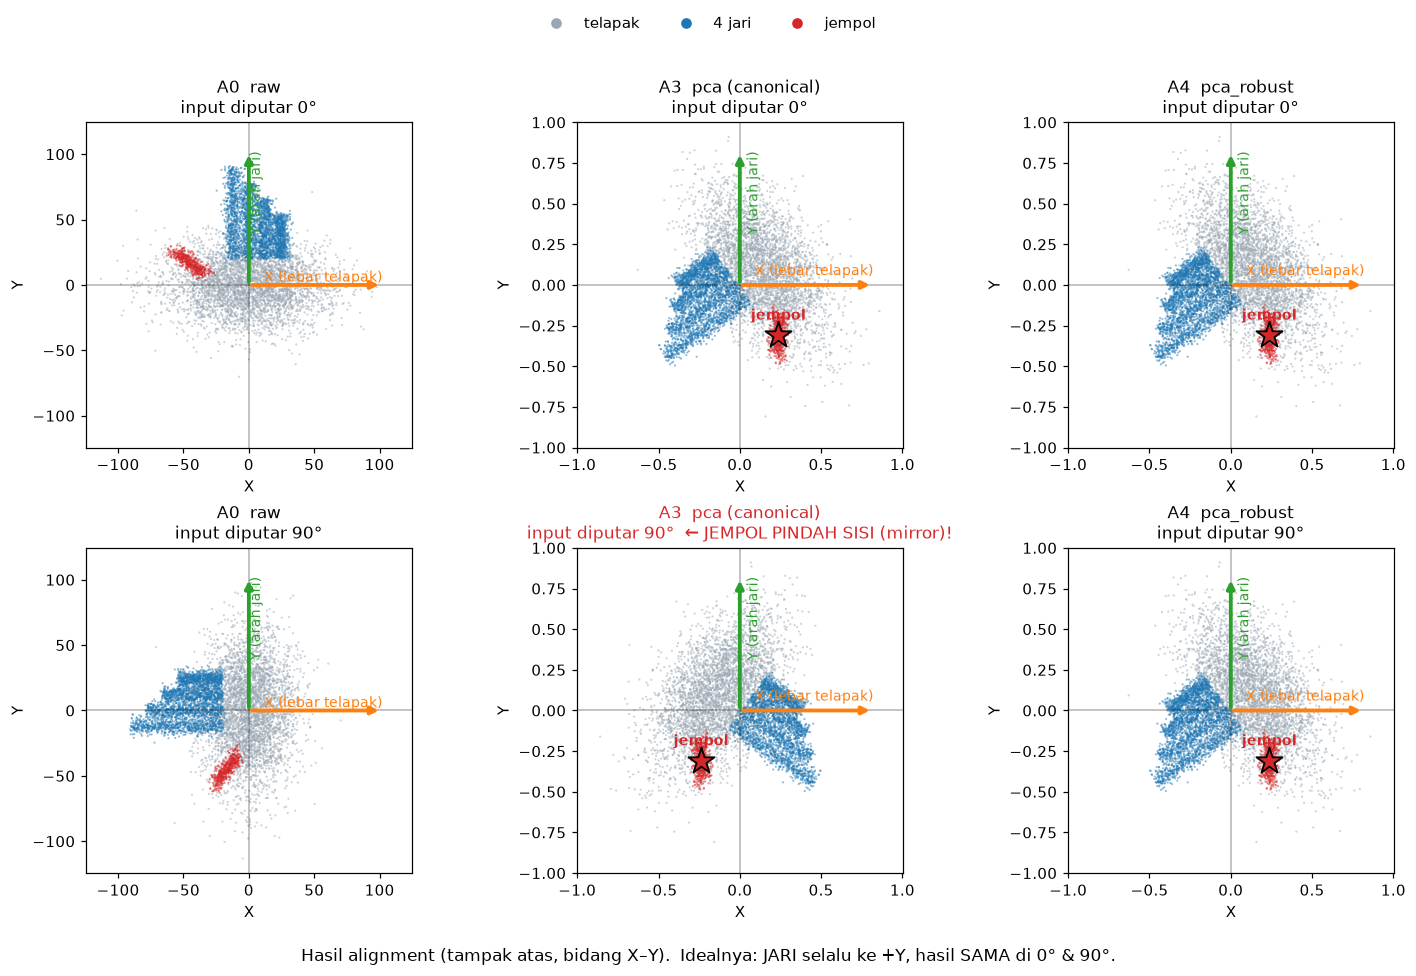
\includegraphics[width=\columnwidth]{figs/alignment_compare.png}
\caption{Alignment of the same hand at input rotations $0^{\circ}$ and
$90^{\circ}$ (top view). The thumb marker (star) tracks chirality. A0 (raw) simply
rotates; A3 (plain PCA) \emph{mirrors} at $90^{\circ}$ (the singularity); A4
(PCA-robust) is identical at $0^{\circ}$ and $90^{\circ}$ (rotation-invariant).}
\label{fig:align}
\end{figure}

\subsection{Factorial accuracy}
Table~\ref{tab:eer} reports EER (\%) for the full grid (heatmap in
Fig.~\ref{fig:heatmap}). The raw baseline (A0) is weakest; all normalized
representations reach near-zero EER at $N{=}M{=}5$. The lower-bound corner is
(A0, softmax) and the deployable operating point is (A4, ArcFace).

\begin{table}[t]
\caption{EER (\%) at $N{=}M{=}5$ (mean\,$\pm$\,std over 5 seeds).}
\label{tab:eer}
\centering
\begin{tabular}{lcc}
\toprule
Representation & Softmax & ArcFace \\
\midrule
A0 raw            & 11.85\,$\pm$\,3.17 & 17.64\,$\pm$\,2.44 \\
A1 center         & 4.58\,$\pm$\,2.09  & 1.45\,$\pm$\,1.19 \\
A2 center+scale   & 0.06\,$\pm$\,0.12  & 0.00\,$\pm$\,0.00 \\
A3 PCA-canonical  & 0.03\,$\pm$\,0.06  & 0.00\,$\pm$\,0.00 \\
A4 PCA-robust     & 1.33\,$\pm$\,1.33  & 0.52\,$\pm$\,0.88 \\
A5 anatomical     & 0.48\,$\pm$\,0.90  & 0.58\,$\pm$\,0.53 \\
\bottomrule
\end{tabular}
\end{table}

\begin{figure}[t]
\centering
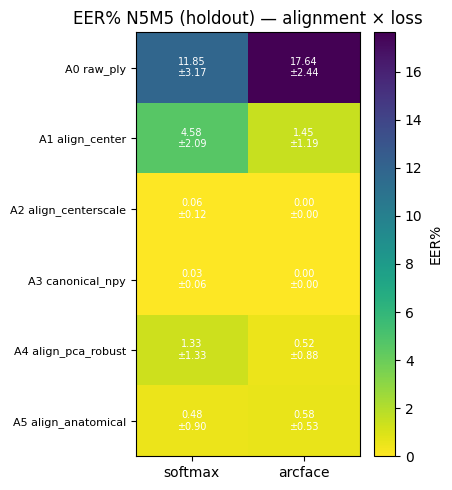
\includegraphics[width=0.8\columnwidth]{figs/eer_heatmap.png}
\caption{Factorial EER (\%) heatmap (alignment $\times$ loss).}
\label{fig:heatmap}
\end{figure}

\subsection{H1: canonicalization and rotation robustness}
We rotate raw probes about the optical axis and re-derive each representation
(Fig.~\ref{fig:rotation}, Table~\ref{tab:rot}). Centering/scaling (A1, A2) do not
align orientation and collapse under rotation; A3 is flat except for a sharp spike
at $90^{\circ}$ (the PCA singularity); \textbf{A4 is flat across all angles}
(EER $\leq 0.9\%$ from $0^{\circ}$ to $180^{\circ}$), and A5 is flat but with a
higher error floor. Thus robustness is not a property of \emph{any} normalization
but specifically of a rotation-stable canonical frame; A4 is the robustness winner
and the recommended representation for deployment.

\begin{table}[t]
\caption{Rotation EER (\%) for ArcFace at key in-plane angles.}
\label{tab:rot}
\centering
\begin{tabular}{lccc}
\toprule
Representation & $0^{\circ}$ & $90^{\circ}$ & $180^{\circ}$ \\
\midrule
A0 raw           & 10.5 & 37.9 & 39.0 \\
A1 center        & 0.8  & 38.8 & 42.7 \\
A2 center+scale  & 0.0  & 35.9 & 36.3 \\
A3 PCA-canonical & 0.0  & \textbf{41.0} & 0.0 \\
A4 PCA-robust    & 0.1  & \textbf{0.7}  & 0.9 \\
A5 anatomical    & 13.9 & 13.6 & 13.8 \\
\bottomrule
\end{tabular}
\end{table}

\begin{figure}[t]
\centering
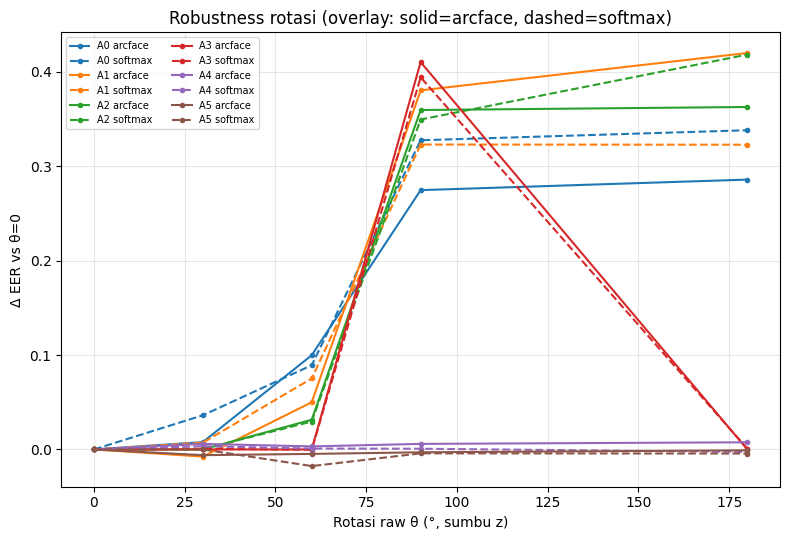
\includegraphics[width=\columnwidth]{figs/rotation.png}
\caption{Rotation sensitivity ($\Delta$EER vs.\ angle). Solid: ArcFace; dashed:
softmax. A3 spikes at $90^{\circ}$; A4 stays flat.}
\label{fig:rotation}
\end{figure}

\subsection{H2: angular margin improves separability}
At $N{=}M{=}5$ the EER on normalized representations is already at the measurement
floor ($\approx 0$), so a paired test on EER is under-powered. We therefore report
the discriminability index $d'$, which retains head-room. Angular margin roughly
\emph{doubles} $d'$ on every normalized representation
(Table~\ref{tab:dprime}), and the improvement is significant for all of
A1--A5 (paired $t$-test over seeds, $p<0.05$); on raw input (A0) the margin does
not help, consistent with the view that ArcFace sharpens an \emph{already
learnable} geometry rather than rescuing an ill-posed one. The t-SNE projections
(Fig.~\ref{fig:tsne}) and the near-diagonal confusion matrix corroborate this.

\begin{table}[t]
\caption{Discriminability $d'$ (mean over seeds); $\Delta$ and paired-test
$p$ for ArcFace vs.\ softmax. Higher $d'$ is better.}
\label{tab:dprime}
\centering
\begin{tabular}{lcccc}
\toprule
Repr. & $d'$ softmax & $d'$ ArcFace & $\Delta$ & $p$ \\
\midrule
A0 raw           & 1.89 & 1.80 & $-0.09$ & 0.574 \\
A1 center        & 3.28 & 6.63 & $+3.34$ & $<0.001$ \\
A2 center+scale  & 4.20 & 9.49 & $+5.28$ & 0.001 \\
A3 PCA-canonical & 4.09 & 8.87 & $+4.78$ & $<0.001$ \\
A4 PCA-robust    & 4.02 & 8.02 & $+4.00$ & $<0.001$ \\
A5 anatomical    & 3.93 & 8.11 & $+4.19$ & 0.003 \\
\bottomrule
\end{tabular}
\end{table}

\begin{figure}[t]
\centering
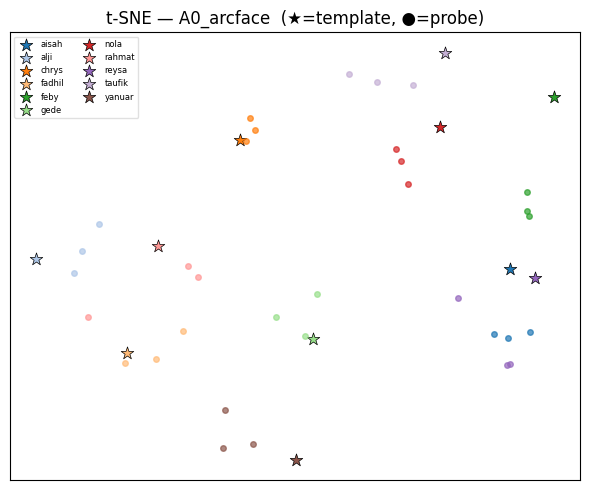
\includegraphics[width=0.49\columnwidth]{figs/tsne_A0.png}\hfill
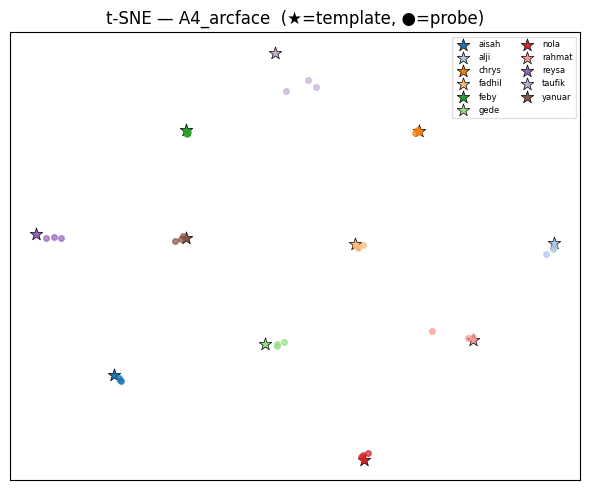
\includegraphics[width=0.49\columnwidth]{figs/tsne_A4.png}
\caption{t-SNE of embeddings (ArcFace). Left: A0 raw (overlapping identities).
Right: A4 PCA-robust (well-separated clusters). Stars: gallery templates; dots:
probes; color: identity.}
\label{fig:tsne}
\end{figure}

\subsection{Discussion}
\textbf{Accuracy vs.\ robustness.} A2/A3 are marginally best at the canonical pose
but collapse under rotation (A3 at $90^{\circ}$); A4 trades a negligible amount of
canonical-pose accuracy for full rotation robustness and is therefore the
preferred operating point. \textbf{Floor effect.} With canonicalization and
multi-frame fusion the EER saturates near zero, so $d'$ (or single-frame EER) is
the appropriate channel to read the margin effect. \textbf{Limitations.} The study
uses $11$ subjects and five seeds; the small cohort and EER quantization limit
external validity, and residual low-level CUDA non-determinism produces negligible
seed-internal variation. Larger cohorts, open-set/cross-dataset tests, and
stronger backbones are left for future work.

% =====================================================================
\section{Conclusion}
% =====================================================================
Treating canonicalization and angular margin as separable factors, a single
PointNet++ encoder achieves near-zero EER for contactless 3D palm recognition. A
deterministic PCA-robust canonicalization removes the $90^{\circ}$ singularity of
plain PCA and delivers rotation-robust recognition, while angular margin roughly
doubles embedding discriminability on every normalized representation. These
results indicate that point-cloud backbones, properly canonicalized and trained
with angular margin, are well suited to 3D palm biometrics.

\bibliographystyle{IEEEtran}
\bibliography{refs}

\end{document}
